% !TeX program = xelatex
\documentclass{article}
\usepackage{kotex}
\usepackage[a4paper,left=3cm, right=3cm, top=2cm, bottom=2cm]{geometry}
\usepackage{amsmath}
\usepackage{graphicx}
\usepackage{caption}
\usepackage{setspace}
\usepackage{xcolor}
\usepackage{titlesec}
\usepackage{amssymb}
\usepackage{tcolorbox}
\usepackage{amsthm}
\usepackage{multirow}
\usepackage{array}
\usepackage{booktabs}
\usepackage{tikz}
\usetikzlibrary{positioning,arrows.meta,calc}
\usepackage{pgfplots}
\pgfplotsset{compat=1.18}

\title{7.5 Hermitian, Unitary, and Normal Matrices}
\date{}
\author{}
\setstretch{1.3}

\titleformat{name=\section, numberless}
  {\normalfont\large\bfseries\color{blue}}{}
  {0pt}{}
\geometry{a4paper, margin=1in}

\newcommand{\redheading}[1]{{\vspace{2mm}\noindent\Large\bfseries\color{red!55!black} #1\par}\vspace{2mm}}

\begin{document}
\maketitle

{\itshape\color{blue!45!black}
In Section~7.2 we showed that every real symmetric matrix is orthogonally diagonalizable,
and conversely every orthogonally diagonalizable real matrix is symmetric.
In this section we extend the diagonalization problem to matrices with complex entries.\par}

\vspace{2mm}

\redheading{Real Matrices Versus Complex Matrices}

We call matrices with real entries \textbf{real matrices} and matrices whose entries may be complex numbers \textbf{complex matrices}. Similarly, vectors in $\mathbb{R}^n$ are \textbf{real vectors} and those in $\mathbb{C}^n$ are \textbf{complex vectors}. Every real matrix is a special case of a complex matrix.

\redheading{Hermitian and Unitary Matrices}

For complex matrices, the transpose is replaced by a more useful operation.

\begin{tcolorbox}[colback=teal!4, colframe=teal!65!black,
  title={\textbf{Definition 1}}, boxrule=0.5mm, arc=3mm]
If $A$ is a complex matrix, the \textbf{conjugate transpose} of $A$, denoted $A^*$, is
\begin{equation}
  A^* = \overline{A}^T
\end{equation}
\end{tcolorbox}

\textit{Remark.} The order of transpose and conjugation does not matter (Theorem~5.3.2b).
If $A$ is real, then $A^* = A^T$.

\subsection*{EXAMPLE 1 | Conjugate Transpose}

Find $A^*$ of
$A = \begin{bmatrix} 1+i & -i & 0 \\ 2 & 3-2i & i \end{bmatrix}$.

\textbf{SOLUTION:}
\[
  \overline{A} = \begin{bmatrix} 1-i & i & 0 \\ 2 & 3+2i & -i \end{bmatrix},
  \qquad
  A^* = \overline{A}^T = \begin{bmatrix} 1-i & 2 \\ i & 3+2i \\ 0 & -i \end{bmatrix}
\]

The following theorem (parts proved in the exercises) shows that the conjugate transpose obeys the same algebraic rules as the ordinary transpose.

\begin{tcolorbox}[colback=red!4, colframe=red!60!black,
  title={\textbf{Theorem 7.5.1}}, boxrule=0.5mm, arc=3mm]
If $k$ is a complex scalar and $A$, $B$ are complex matrices of compatible sizes, then:
\begin{enumerate}
  \item[(a)] $(A^*)^* = A$
  \item[(b)] $(A+B)^* = A^*+B^*$
  \item[(c)] $(A-B)^* = A^*-B^*$
  \item[(d)] $(kA)^* = \bar{k}A^*$
  \item[(e)] $(AB)^* = B^*A^*$
\end{enumerate}
\end{tcolorbox}

\begin{tcolorbox}[colback=teal!4, colframe=teal!65!black,
  title={\textbf{Definition 2}}, boxrule=0.5mm, arc=3mm]
A square matrix $A$ is \textbf{unitary} if
\begin{equation}
  AA^* = A^*A = I
\end{equation}
or equivalently $A^* = A^{-1}$, and it is \textbf{Hermitian}\footnotemark{} if
\begin{equation}
  A^* = A
\end{equation}
\end{tcolorbox}
\footnotetext{Named for the French mathematician Charles Hermite (1822--1901).}

If $A$ is real, unitary reduces to orthogonal and Hermitian reduces to symmetric.
To show a matrix is unitary, it suffices to verify $AA^* = I$ or $A^*A = I$ (either implies the other).

\subsection*{EXAMPLE 2 | Recognizing Hermitian Matrices}

A Hermitian matrix has real diagonal entries and conjugate-symmetric off-diagonal entries.
By inspection, the following matrix is Hermitian:
\[
  A = \begin{bmatrix} 1 & i & 1+i \\ -i & -5 & 2-i \\ 1-i & 2+i & 3 \end{bmatrix}
\]

\subsection*{EXAMPLE 3 | Recognizing Unitary Matrices}

Unitary matrices are not easy to identify by inspection; the most direct way is to check
Equation~(2) or (3). We leave it to the reader to verify that
\[
  A = \begin{bmatrix} \tfrac{1}{\sqrt{2}} & -\tfrac{i}{\sqrt{2}} \\ -\tfrac{i}{\sqrt{2}} & \tfrac{1}{\sqrt{2}} \end{bmatrix}
\]
is unitary.

Recall from Section~5.3 that the complex Euclidean inner product on $\mathbb{C}^n$ satisfies
\begin{equation}
  \mathbf{u}\cdot\mathbf{v} = \mathbf{v}^*\mathbf{u}
\end{equation}
We use this to prove the following theorem (a complex analog of Theorem~7.2.2).

\begin{tcolorbox}[colback=red!4, colframe=red!60!black,
  title={\textbf{Theorem 7.5.2}}, boxrule=0.5mm, arc=3mm]
If $A$ is Hermitian, then:
\begin{enumerate}
  \item[(a)] The eigenvalues of $A$ are real.
  \item[(b)] Eigenvectors from different eigenspaces are orthogonal.
\end{enumerate}

\medskip
\textbf{Proof of (b).} Let $\mathbf{v}_1,\mathbf{v}_2$ be eigenvectors for distinct eigenvalues
$\lambda_1,\lambda_2$. Since the eigenvalues are real ($\lambda_i = \bar{\lambda}_i$) and $A = A^*$,
using Formula~(5):
\[
  \lambda_1(\mathbf{v}_2\cdot\mathbf{v}_1)
  = (\lambda_1\mathbf{v}_1)^*\mathbf{v}_2
  = (A\mathbf{v}_1)^*\mathbf{v}_2
  = (\mathbf{v}_1^*A^*)\mathbf{v}_2
  = \mathbf{v}_1^*(A\mathbf{v}_2)
  = \mathbf{v}_1^*(\lambda_2\mathbf{v}_2)
  = \lambda_2(\mathbf{v}_2\cdot\mathbf{v}_1)
\]
Thus $(\lambda_1-\lambda_2)(\mathbf{v}_2\cdot\mathbf{v}_1)=0$, and since $\lambda_1\neq\lambda_2$,
we have $\mathbf{v}_2\cdot\mathbf{v}_1 = 0$.\quad$\blacksquare$
\end{tcolorbox}

\subsection*{EXAMPLE 4 | Eigenvalues and Eigenvectors of a Hermitian Matrix}

Confirm that
$A = \begin{bmatrix} 2 & 1+i \\ 1-i & 3 \end{bmatrix}$
has real eigenvalues and that eigenvectors from different eigenspaces are orthogonal.

\textbf{SOLUTION:}
\[
  \det(\lambda I - A) = \begin{vmatrix} \lambda-2 & -1-i \\ -1+i & \lambda-3 \end{vmatrix}
  = (\lambda-2)(\lambda-3)-(-1-i)(-1+i) = \lambda^2-5\lambda+4 = (\lambda-1)(\lambda-4)
\]
The eigenvalues are $\lambda=1$ and $\lambda=4$, both real. Solving $(\lambda I-A)\mathbf{x}=\mathbf{0}$:
\[
  \lambda=1:\quad \mathbf{v}_1 = \begin{bmatrix}-1-i\\1\end{bmatrix},
  \qquad
  \lambda=4:\quad \mathbf{v}_2 = \begin{bmatrix}\tfrac{1}{2}(1+i)\\1\end{bmatrix}
\]
Orthogonality check:
\[
  \mathbf{v}_1\cdot\mathbf{v}_2 = \overline{(-1-i)}\cdot\tfrac{1}{2}(1+i) + \overline{1}\cdot 1
  = (-1+i)\cdot\tfrac{1}{2}(1+i)+1 = \tfrac{1}{2}(-1+i)(1+i)+1 = \tfrac{1}{2}(-2)+1 = 0 \checkmark
\]

\begin{tcolorbox}[colback=red!4, colframe=red!60!black,
  title={\textbf{Theorem 7.5.3}}, boxrule=0.5mm, arc=3mm]
If $A$ is an $n\times n$ complex matrix, the following are equivalent:
\begin{enumerate}
  \item[(a)] $A$ is unitary.
  \item[(b)] $\|A\mathbf{x}\|=\|\mathbf{x}\|$ for all $\mathbf{x}$ in $\mathbb{C}^n$.
  \item[(c)] $A\mathbf{x}\cdot A\mathbf{y} = \mathbf{x}\cdot\mathbf{y}$ for all $\mathbf{x},\mathbf{y}$ in $\mathbb{C}^n$.
  \item[(d)] The column vectors of $A$ form an orthonormal set in $\mathbb{C}^n$.
  \item[(e)] The row vectors of $A$ form an orthonormal set in $\mathbb{C}^n$.
\end{enumerate}
\end{tcolorbox}

\redheading{Unitary Diagonalizability}

Since unitary matrices are the complex analogs of real orthogonal matrices, the following definition naturally generalizes orthogonal diagonalizability.

\begin{tcolorbox}[colback=teal!4, colframe=teal!65!black,
  title={\textbf{Definition 3}}, boxrule=0.5mm, arc=3mm]
A square complex matrix $A$ is \textbf{unitarily diagonalizable} if there is a unitary
matrix $P$ such that $P^*AP = D$ is a complex diagonal matrix. Any such $P$
\textbf{unitarily diagonalizes} $A$.
\end{tcolorbox}

\subsection*{EXAMPLE 5 | A Unitary Matrix}

Show that
$A = \begin{bmatrix} \tfrac{1}{2}(1+i) & \tfrac{1}{2}(1+i) \\ \tfrac{1}{2}(1-i) & \tfrac{1}{2}(-1+i) \end{bmatrix}$
is unitary and find $A^{-1}$.

\textbf{SOLUTION:}
We verify orthonormality of rows. With
$\mathbf{r}_1 = \bigl[\tfrac{1}{2}(1+i),\;\tfrac{1}{2}(1+i)\bigr]$
and
$\mathbf{r}_2 = \bigl[\tfrac{1}{2}(1-i),\;\tfrac{1}{2}(-1+i)\bigr]$:
\begin{align*}
  \|\mathbf{r}_1\| &= \sqrt{\bigl|\tfrac{1}{2}(1+i)\bigr|^2+\bigl|\tfrac{1}{2}(1+i)\bigr|^2} = \sqrt{\tfrac{1}{2}+\tfrac{1}{2}} = 1 \\
  \|\mathbf{r}_2\| &= \sqrt{\bigl|\tfrac{1}{2}(1-i)\bigr|^2+\bigl|\tfrac{1}{2}(-1+i)\bigr|^2} = \sqrt{\tfrac{1}{2}+\tfrac{1}{2}} = 1 \\
  \mathbf{r}_1\cdot\mathbf{r}_2 &= \bigl(\tfrac{1}{2}(1+i)\bigr)\overline{\bigl(\tfrac{1}{2}(1-i)\bigr)}
                                    +\bigl(\tfrac{1}{2}(1+i)\bigr)\overline{\bigl(\tfrac{1}{2}(-1+i)\bigr)} \\
                                 &= \bigl(\tfrac{1}{2}(1+i)\bigr)\bigl(\tfrac{1}{2}(1+i)\bigr)
                                    +\bigl(\tfrac{1}{2}(1+i)\bigr)\bigl(\tfrac{1}{2}(-1-i)\bigr)
                                  = \tfrac{1}{2}i - \tfrac{1}{2}i = 0
\end{align*}
Since $A$ is unitary, $A^{-1} = A^* = \begin{bmatrix} \tfrac{1}{2}(1-i) & \tfrac{1}{2}(1+i) \\ \tfrac{1}{2}(1-i) & \tfrac{1}{2}(-1-i) \end{bmatrix}$.

The following theorem is the complex analog of Theorems~7.2.1 and 7.2.3.

\begin{tcolorbox}[colback=red!4, colframe=red!60!black,
  title={\textbf{Theorem 7.5.4}}, boxrule=0.5mm, arc=3mm]
Every $n\times n$ Hermitian matrix $A$ has an orthonormal set of $n$ eigenvectors.
Moreover, $A$ is unitarily diagonalized by any $n\times n$ matrix $P$ whose column vectors
form an orthonormal set of eigenvectors of $A$.
\end{tcolorbox}

The procedure for unitarily diagonalizing a Hermitian matrix is exactly the same as for orthogonal diagonalization of a symmetric matrix.

\begin{tcolorbox}[colback=teal!4, colframe=teal!65!black,
  title={\textbf{Unitarily Diagonalizing a Hermitian Matrix}}, boxrule=0.5mm, arc=3mm]
\textbf{Step 1.} Find a basis for each eigenspace of $A$.\\[4pt]
\textbf{Step 2.} Apply the Gram--Schmidt process to each basis to obtain orthonormal bases
for the eigenspaces.\\[4pt]
\textbf{Step 3.} Form the matrix $P$ whose columns are the orthonormal basis vectors from
Step~2. By Theorem~7.5.3, $P$ is unitary and $P^*AP$ is diagonal.
\end{tcolorbox}

\subsection*{EXAMPLE 6 | Unitary Diagonalization of a Hermitian Matrix}

Find a matrix $P$ that unitarily diagonalizes
$A = \begin{bmatrix} 2 & 1+i \\ 1-i & 3 \end{bmatrix}$.

\textbf{SOLUTION:}
From Example~4, the eigenvalues are $\lambda=1$ and $\lambda=4$ with eigenvectors
$\mathbf{v}_1 = \begin{bmatrix}-1-i\\1\end{bmatrix}$
and
$\mathbf{v}_2 = \begin{bmatrix}\tfrac{1}{2}(1+i)\\1\end{bmatrix}$.
Normalizing:
\[
  \|\mathbf{v}_1\| = \sqrt{|{-1-i}|^2+1} = \sqrt{3},
  \qquad
  \|\mathbf{v}_2\| = \sqrt{\bigl|\tfrac{1}{2}(1+i)\bigr|^2+1} = \sqrt{\tfrac{1}{2}+1} = \sqrt{\tfrac{3}{2}}
\]
\[
  \mathbf{p}_1 = \frac{\mathbf{v}_1}{\|\mathbf{v}_1\|} = \begin{bmatrix}\dfrac{-1-i}{\sqrt{3}}\\[4pt]\dfrac{1}{\sqrt{3}}\end{bmatrix},
  \qquad
  \mathbf{p}_2 = \frac{\mathbf{v}_2}{\|\mathbf{v}_2\|} = \begin{bmatrix}\dfrac{1+i}{\sqrt{6}}\\[4pt]\dfrac{2}{\sqrt{6}}\end{bmatrix}
\]
Thus $A$ is unitarily diagonalized by
\[
  P = \begin{bmatrix} \dfrac{-1-i}{\sqrt{3}} & \dfrac{1+i}{\sqrt{6}} \\[6pt] \dfrac{1}{\sqrt{3}} & \dfrac{2}{\sqrt{6}} \end{bmatrix},
  \qquad
  P^*AP = \begin{bmatrix} 1 & 0 \\ 0 & 4 \end{bmatrix}
\]

\redheading{Skew-Symmetric and Skew-Hermitian Matrices}

Two more matrix classes arise naturally in the diagonalization problem. A square real matrix $A$ is \textbf{skew-symmetric} if $A^T = -A$, and a square complex matrix $A$ is \textbf{skew-Hermitian} if $A^* = -A$. It can be shown that a skew-symmetric matrix must have zeros on the main diagonal, while a skew-Hermitian matrix must have zeros or pure imaginary numbers on the main diagonal. Examples:
\[
  A = \begin{bmatrix} 0 & 1 & -2 \\ -1 & 0 & 4 \\ 2 & -4 & 0 \end{bmatrix}
  \quad\text{[skew-symmetric]},
  \qquad
  A = \begin{bmatrix} i & 1-i & 5 \\ -1-i & 2i & i \\ -5 & i & 0 \end{bmatrix}
  \quad\text{[skew-Hermitian]}
\]

\redheading{Normal Matrices}

Hermitian matrices are unitarily diagonalizable, but they do not exhaust the class of unitarily diagonalizable complex matrices. It can be proved that a square complex matrix $A$ is unitarily diagonalizable if and only if
\begin{equation}
  AA^* = A^*A
\end{equation}
Matrices satisfying (6) are called \textbf{normal}. Normal matrices include Hermitian, skew-Hermitian, and unitary matrices in the complex case, and symmetric, skew-symmetric, and orthogonal matrices in the real case.

\textit{Note.} Nonzero skew-symmetric matrices are interesting because they are real matrices that are not orthogonally diagonalizable but are unitarily diagonalizable.

\redheading{A Comparison of Eigenvalues}

Hermitian matrices have real eigenvalues; skew-Hermitian matrices have eigenvalues that are zero or purely imaginary; unitary matrices have eigenvalues with modulus~1. These facts are illustrated in Figure~7.5.1.

\begin{figure}[ht]
\centering
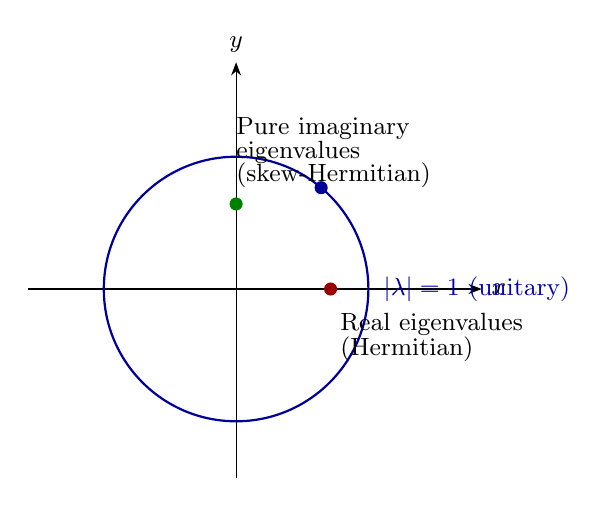
\begin{tikzpicture}[>=Stealth, scale=1.2]
  % Axes
  \draw[->] (-2.2,0) -- (2.6,0) node[right, font=\small] {$x$};
  \draw[->] (0,-2.0) -- (0,2.4) node[above, font=\small] {$y$};
  % Unit circle
  \draw[thick, blue!60!black] (0,0) circle (1.4cm);
  % Labels on circle
  \node[blue!70!black, font=\small] at (1.4, 0) [right=2pt] {$|\lambda|=1$ (unitary)};
  % Real axis label
  \node[font=\small, below right] at (1.0, -0.15) {Real eigenvalues};
  \node[font=\small, below right] at (1.0, -0.40) {(Hermitian)};
  % Imaginary axis label
  \node[font=\small, align=left] at (-0.1, 1.7) [right] {Pure imaginary};
  \node[font=\small, align=left] at (-0.1, 1.45) [right] {eigenvalues};
  \node[font=\small, align=left] at (-0.1, 1.20) [right] {(skew-Hermitian)};
  % Dots indicating eigenvalue positions
  \filldraw[red!60!black] (1.0, 0) circle (1.8pt);
  \filldraw[green!50!black] (0, 0.9) circle (1.8pt);
  \filldraw[blue!60!black] ({1.4*cos(50)}, {1.4*sin(50)}) circle (1.8pt);
\end{tikzpicture}
\caption*{FIGURE 7.5.1\quad Eigenvalue locations for Hermitian, skew-Hermitian, and unitary matrices.}
\end{figure}

\vspace{3mm}
\noindent\rule{\linewidth}{0.5pt}

\section*{Exercise Set 7.5}

\noindent\textit{In Exercises 1--2, find $A^*$.}

\begin{enumerate}
  \item[(1)] $A = \begin{bmatrix} 2i & 1-i \\ 4 & 3+i \\ 5+i & 0 \end{bmatrix}$

  \item[(3)] Substitute numbers for the $\times$'s so that $A$ is Hermitian:
  $A = \begin{bmatrix} 1 & i & 2-3i \\ \times & -3 & 1 \\ \times & \times & 2 \end{bmatrix}$

  \item[(5)] \textbf{a.} Show that $A$ is not Hermitian for any choice of the $\times$'s:
  $A = \begin{bmatrix} 1 & i & 2-3i \\ -i & -3 & \times \\ 2-3i & \times & \times \end{bmatrix}$

  \item[(7)] Verify that the eigenvalues of the Hermitian matrix are real and that
  eigenvectors from different eigenspaces are orthogonal (see Theorem~7.5.2):
  $A = \begin{bmatrix} 3 & 2-3i \\ 2+3i & -1 \end{bmatrix}$

  \item[(9)] Show that $A$ is unitary and find $A^{-1}$:
  $A = \begin{bmatrix} \tfrac{3}{5} & \tfrac{4}{5}i \\ -\tfrac{4}{5} & \tfrac{3}{5}i \end{bmatrix}$

  \item[(11)] Show that $A$ is unitary and find $A^{-1}$:
  $A = \dfrac{1}{2\sqrt{2}}\begin{bmatrix} \sqrt{3}+i & 1-i\sqrt{3} \\ 1+i\sqrt{3} & i-\sqrt{3} \end{bmatrix}$
\end{enumerate}

\noindent\textit{In Exercises 13--18, find a unitary matrix $P$ that diagonalizes $A$, and determine $P^{-1}AP$.}

\begin{enumerate}
  \item[(13)] $A = \begin{bmatrix} 4 & 1-i \\ 1+i & 5 \end{bmatrix}$

  \item[(15)] $A = \begin{bmatrix} 6 & 2+2i \\ 2-2i & 4 \end{bmatrix}$

  \item[(17)] $A = \begin{bmatrix} 5 & 0 & 0 \\ 0 & -1 & -1+i \\ 0 & -1-i & 0 \end{bmatrix}$
\end{enumerate}

\noindent\textit{In Exercise 19, substitute numbers for the $\times$'s so that $A$ is skew-Hermitian.}

\begin{enumerate}
  \item[(19)] $A = \begin{bmatrix} 0 & i & 2-3i \\ \times & 0 & 1 \\ \times & \times & 4i \end{bmatrix}$
\end{enumerate}

\noindent\textit{In Exercise 23, verify that the eigenvalues of the skew-Hermitian matrix are pure imaginary.}

\begin{enumerate}
  \item[(23)] $A = \begin{bmatrix} 0 & -1+i \\ 1+i & i \end{bmatrix}$
\end{enumerate}

\noindent\textit{In Exercise 25, show that $A$ is normal.}

\begin{enumerate}
  \item[(25)] $A = \begin{bmatrix} 1+2i & 2+i & -2-i \\ 2+i & 1+i & -i \\ -2-i & -i & 1+i \end{bmatrix}$
\end{enumerate}

\begin{enumerate}
  \item[(27)] Let $A$ be any $n\times n$ matrix with complex entries, and define
  $B = \tfrac{1}{2}(A+A^*)$ and $C = \tfrac{1}{2i}(A-A^*)$.
  \begin{enumerate}
    \item[(a)] Show that $B$ and $C$ are Hermitian.
    \item[(b)] Show that $A = B+iC$ and $A^* = B-iC$.
    \item[(c)] What condition must $B$ and $C$ satisfy for $A$ to be normal?
  \end{enumerate}

  \item[(28)] Show that if $A$ is an $n\times n$ matrix with complex entries and
  $\mathbf{u},\mathbf{v}\in\mathbb{C}^n$ are column vectors, then
  \[A\mathbf{u}\cdot\mathbf{v} = \mathbf{u}\cdot A^*\mathbf{v} \qquad\text{and}\qquad \mathbf{u}\cdot A\mathbf{v} = A^*\mathbf{u}\cdot\mathbf{v}\]

  \item[(33)] Under what conditions is the matrix
  $A = \begin{bmatrix} a & 0 & 0 \\ 0 & 0 & c \\ 0 & b & 0 \end{bmatrix}$
  normal?

  \item[(35)] Find a $2\times 2$ matrix that is both Hermitian and unitary and whose entries are not all real numbers.
\end{enumerate}


\end{document}
